% =====================================================================
% 셀프사진관 시장 분석 및 IP 협업 수익 예측 — 요약 보고서
% Compiled with: xelatex photoism_summary.tex
% =====================================================================
\documentclass[11pt, a4paper]{article}

% --- Fonts & Language ---
\usepackage{fontspec}
\usepackage{xetexko}

% --- Page geometry ---
\usepackage[margin=2.3cm, top=2.8cm, bottom=2.8cm]{geometry}

% --- Packages ---
\usepackage{graphicx}
\usepackage{booktabs}
\usepackage{tabularx}
\usepackage{xcolor}
\usepackage{hyperref}
\usepackage{titlesec}
\usepackage{fancyhdr}
\usepackage{float}
\usepackage{enumitem}
\usepackage{colortbl}
\usepackage{tikz}
\usepackage{setspace}
\usepackage{ragged2e}

% --- Font ---
\setmainfont{Apple SD Gothic Neo}

% --- Colors ---
\definecolor{darkblue}{HTML}{0F172A}
\definecolor{lightblue}{HTML}{D4E6F1}
\definecolor{accent}{HTML}{60A5FA}
\definecolor{red}{HTML}{DC2626}
\definecolor{gray}{HTML}{64748B}
\definecolor{kpibox}{HTML}{EBF5FB}
\definecolor{warnbox}{HTML}{FEF3C7}
\definecolor{greenbox}{HTML}{D1FAE5}
\definecolor{lightgray}{HTML}{F1F5F9}
\definecolor{bordergray}{HTML}{CBD5E1}
\definecolor{darkaccent}{HTML}{1E40AF}

% --- Hyperref ---
\hypersetup{
  colorlinks=true,
  linkcolor=darkaccent,
  urlcolor=accent,
  citecolor=darkblue,
  pdfborder={0 0 0}
}

% --- Section formatting ---
\titleformat{\section}
  {\Large\bfseries\color{darkblue}}
  {\thesection}{1em}{}
  [\vspace{-0.5em}\textcolor{accent}{\rule{\textwidth}{1.5pt}}]

\titleformat{\subsection}
  {\large\bfseries\color{darkblue}}
  {\thesubsection}{0.8em}{}

% --- Header / Footer ---
\pagestyle{fancy}
\fancyhf{}
\renewcommand{\headrulewidth}{0pt}
\fancyfoot[C]{\footnotesize\textcolor{gray}{한양대학교 경영대학 임보람 교수 연구실 \textperiodcentered{} 빅데이터 마케팅 연구그룹}}
\fancyfoot[R]{\footnotesize\textcolor{gray}{\thepage}}
\fancypagestyle{plain}{
  \fancyhf{}
  \renewcommand{\headrulewidth}{0pt}
  \fancyfoot[C]{\footnotesize\textcolor{gray}{한양대학교 경영대학 임보람 교수 연구실 \textperiodcentered{} 빅데이터 마케팅 연구그룹}}
  \fancyfoot[R]{\footnotesize\textcolor{gray}{\thepage}}
}

% --- Custom commands ---
\newcommand{\metriccard}[3]{%
  \begin{tikzpicture}
    \node[
      fill=kpibox,
      rounded corners=6pt,
      minimum width=4.8cm,
      minimum height=2.4cm,
      inner sep=8pt,
      align=center
    ] {
      {\small\textcolor{gray}{#1}}\\[3pt]
      {\LARGE\bfseries\textcolor{darkblue}{#2}}\\[2pt]
      {\footnotesize\textcolor{accent}{#3}}
    };
  \end{tikzpicture}%
}

\newcommand{\insightbox}[1]{%
  \vspace{0.5em}
  \noindent
  \fcolorbox{accent}{kpibox}{%
    \parbox{\dimexpr\textwidth-2\fboxsep-2\fboxrule}{%
      \vspace{0.4em}
      \textcolor{darkblue}{\textbf{핵심 인사이트}} \quad #1
      \vspace{0.4em}
    }%
  }%
  \vspace{0.5em}
}

\begin{document}

% =====================================================================
% COVER PAGE
% =====================================================================
\thispagestyle{empty}
\begin{tikzpicture}[remember picture, overlay]
  \fill[darkblue] (current page.north west) rectangle (current page.south east);
  \fill[accent] ([yshift=-9cm]current page.north west) rectangle ([yshift=-9.15cm]current page.north east);
  \fill[accent, opacity=0.3] ([yshift=3cm]current page.south west) rectangle ([yshift=3.08cm]current page.south east);
\end{tikzpicture}

\vspace*{4.5cm}

\begin{center}
  {\fontsize{30}{38}\selectfont\bfseries\textcolor{white}{셀프사진관 시장 분석 및}}\\[0.4cm]
  {\fontsize{30}{38}\selectfont\bfseries\textcolor{white}{IP 협업 수익 예측}}\\[0.8cm]
  {\fontsize{18}{26}\selectfont\bfseries\textcolor{accent}{시장 구조, 성장 지속성, 매출 예측 모델}}\\[1.5cm]
  \textcolor{accent}{\rule{8cm}{0.8pt}}\\[1.5cm]
  {\fontsize{13}{18}\selectfont\textcolor{lightblue}{포토이즘 시장점유율 71.2\% 달성 과정 실증 분석}}\\[0.3cm]
  {\fontsize{13}{18}\selectfont\textcolor{lightblue}{MAPE 2.3\% 매출 예측 및 폐업 예측 AUC 0.991}}\\[2.5cm]
  {\fontsize{12}{16}\selectfont\textcolor{white}{한양대학교 경영대학}}\\[0.3cm]
  {\fontsize{13}{18}\selectfont\bfseries\textcolor{accent}{임보람 교수 연구실}}\\[0.3cm]
  {\fontsize{11}{15}\selectfont\textcolor{lightblue}{빅데이터 마케팅 연구그룹}}\\[2cm]
  {\footnotesize\textcolor{gray}{Summary Report}}
\end{center}

\newpage

% =====================================================================
% PAGE 2: EXECUTIVE SUMMARY
% =====================================================================
\section*{Executive Summary}

\vspace{0.5em}

셀프사진관 시장은 일시적 유행이 아닌 \textbf{구조적 성장 산업}이며, 포토이즘은 시장점유율 \textbf{71.2\%}로 압도적 1위를 달성했다. 본 연구는 매출 예측, 폐업 예측, IP 협업 효과 분석을 통해 셀프사진관 산업의 미래를 실증적으로 분석한다.

\vspace{1em}

\begin{center}
\metriccard{시장점유율}{71.2\%}{포토이즘 업계 1위}
\hfill
\metriccard{매출 예측 정확도}{MAPE 2.3\%}{월별 매출 예측 모델}
\hfill
\metriccard{폐업 예측 AUC}{0.991}{경쟁사 폐업 사전 감지}
\end{center}

\vspace{1em}

\insightbox{포토이즘은 2021년 인생네컷을 시장점유율에서 역전한 후, 지속적으로 격차를 확대하며 압도적 시장 지배력을 구축했다. 매출 예측 모델은 MAPE 2.3\%로 거의 완벽한 정확도를 보이며, 폐업 예측 모델(AUC 0.991)은 경쟁사의 폐업을 사전에 감지할 수 있다.}

\vspace{1em}

\subsection*{분석 규모}
\begin{itemize}[leftmargin=1.5em, itemsep=3pt]
  \item 전국 셀프사진관 \textbf{전수 데이터} 분석
  \item 포토이즘, 인생네컷 등 주요 브랜드 시계열 추적
  \item IP 콜라보레이션 매출 증분 효과 정밀 측정
\end{itemize}

\newpage

% =====================================================================
% PAGE 3: 시장 점유율 역전
% =====================================================================
\section*{시장 점유율 역전: 포토이즘의 부상}

\vspace{0.5em}

포토이즘은 후발주자로 시작했지만, \textbf{2021년을 기점으로 인생네컷을 역전}하며 시장 1위로 올라섰다. 이후 격차는 지속적으로 확대되어 현재 \textbf{71.2\%}의 압도적 점유율을 기록하고 있다.

\vspace{1em}

\begin{figure}[H]
  \centering
  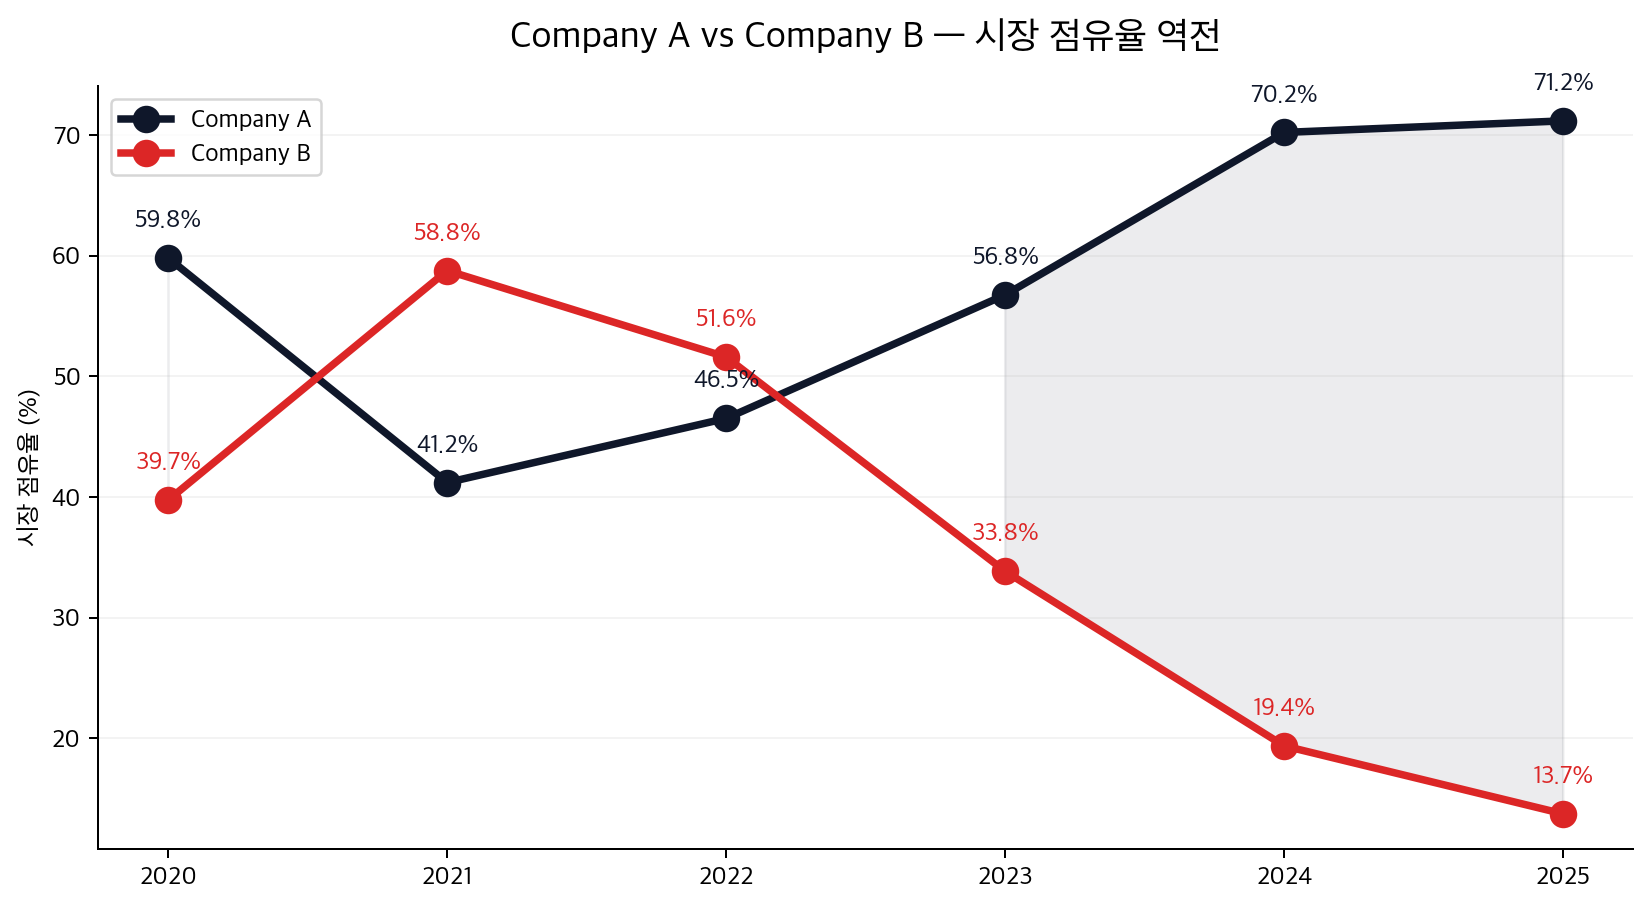
\includegraphics[width=0.92\textwidth]{B5_market_share_crossover.png}
  \caption{포토이즘 vs 인생네컷 시장점유율 역전 추이}
\end{figure}

\vspace{0.5em}

\insightbox{포토이즘의 성장은 단순한 매장 수 확대가 아닌, 브랜드 파워와 IP 협업 전략에 기반한 \textbf{질적 성장}이다. 인생네컷 대비 매장당 매출이 높으며, 폐업률은 낮다.}

\newpage

% =====================================================================
% PAGE 4: Fad 반박 6가지 증거
% =====================================================================
\section*{일시적 유행이 아닌 6가지 증거}

\vspace{0.5em}

셀프사진관 시장이 ``유행''에 불과하다는 우려에 대해, 본 연구는 \textbf{6가지 실증적 증거}를 통해 이를 체계적으로 반박한다.

\vspace{1em}

\begin{figure}[H]
  \centering
  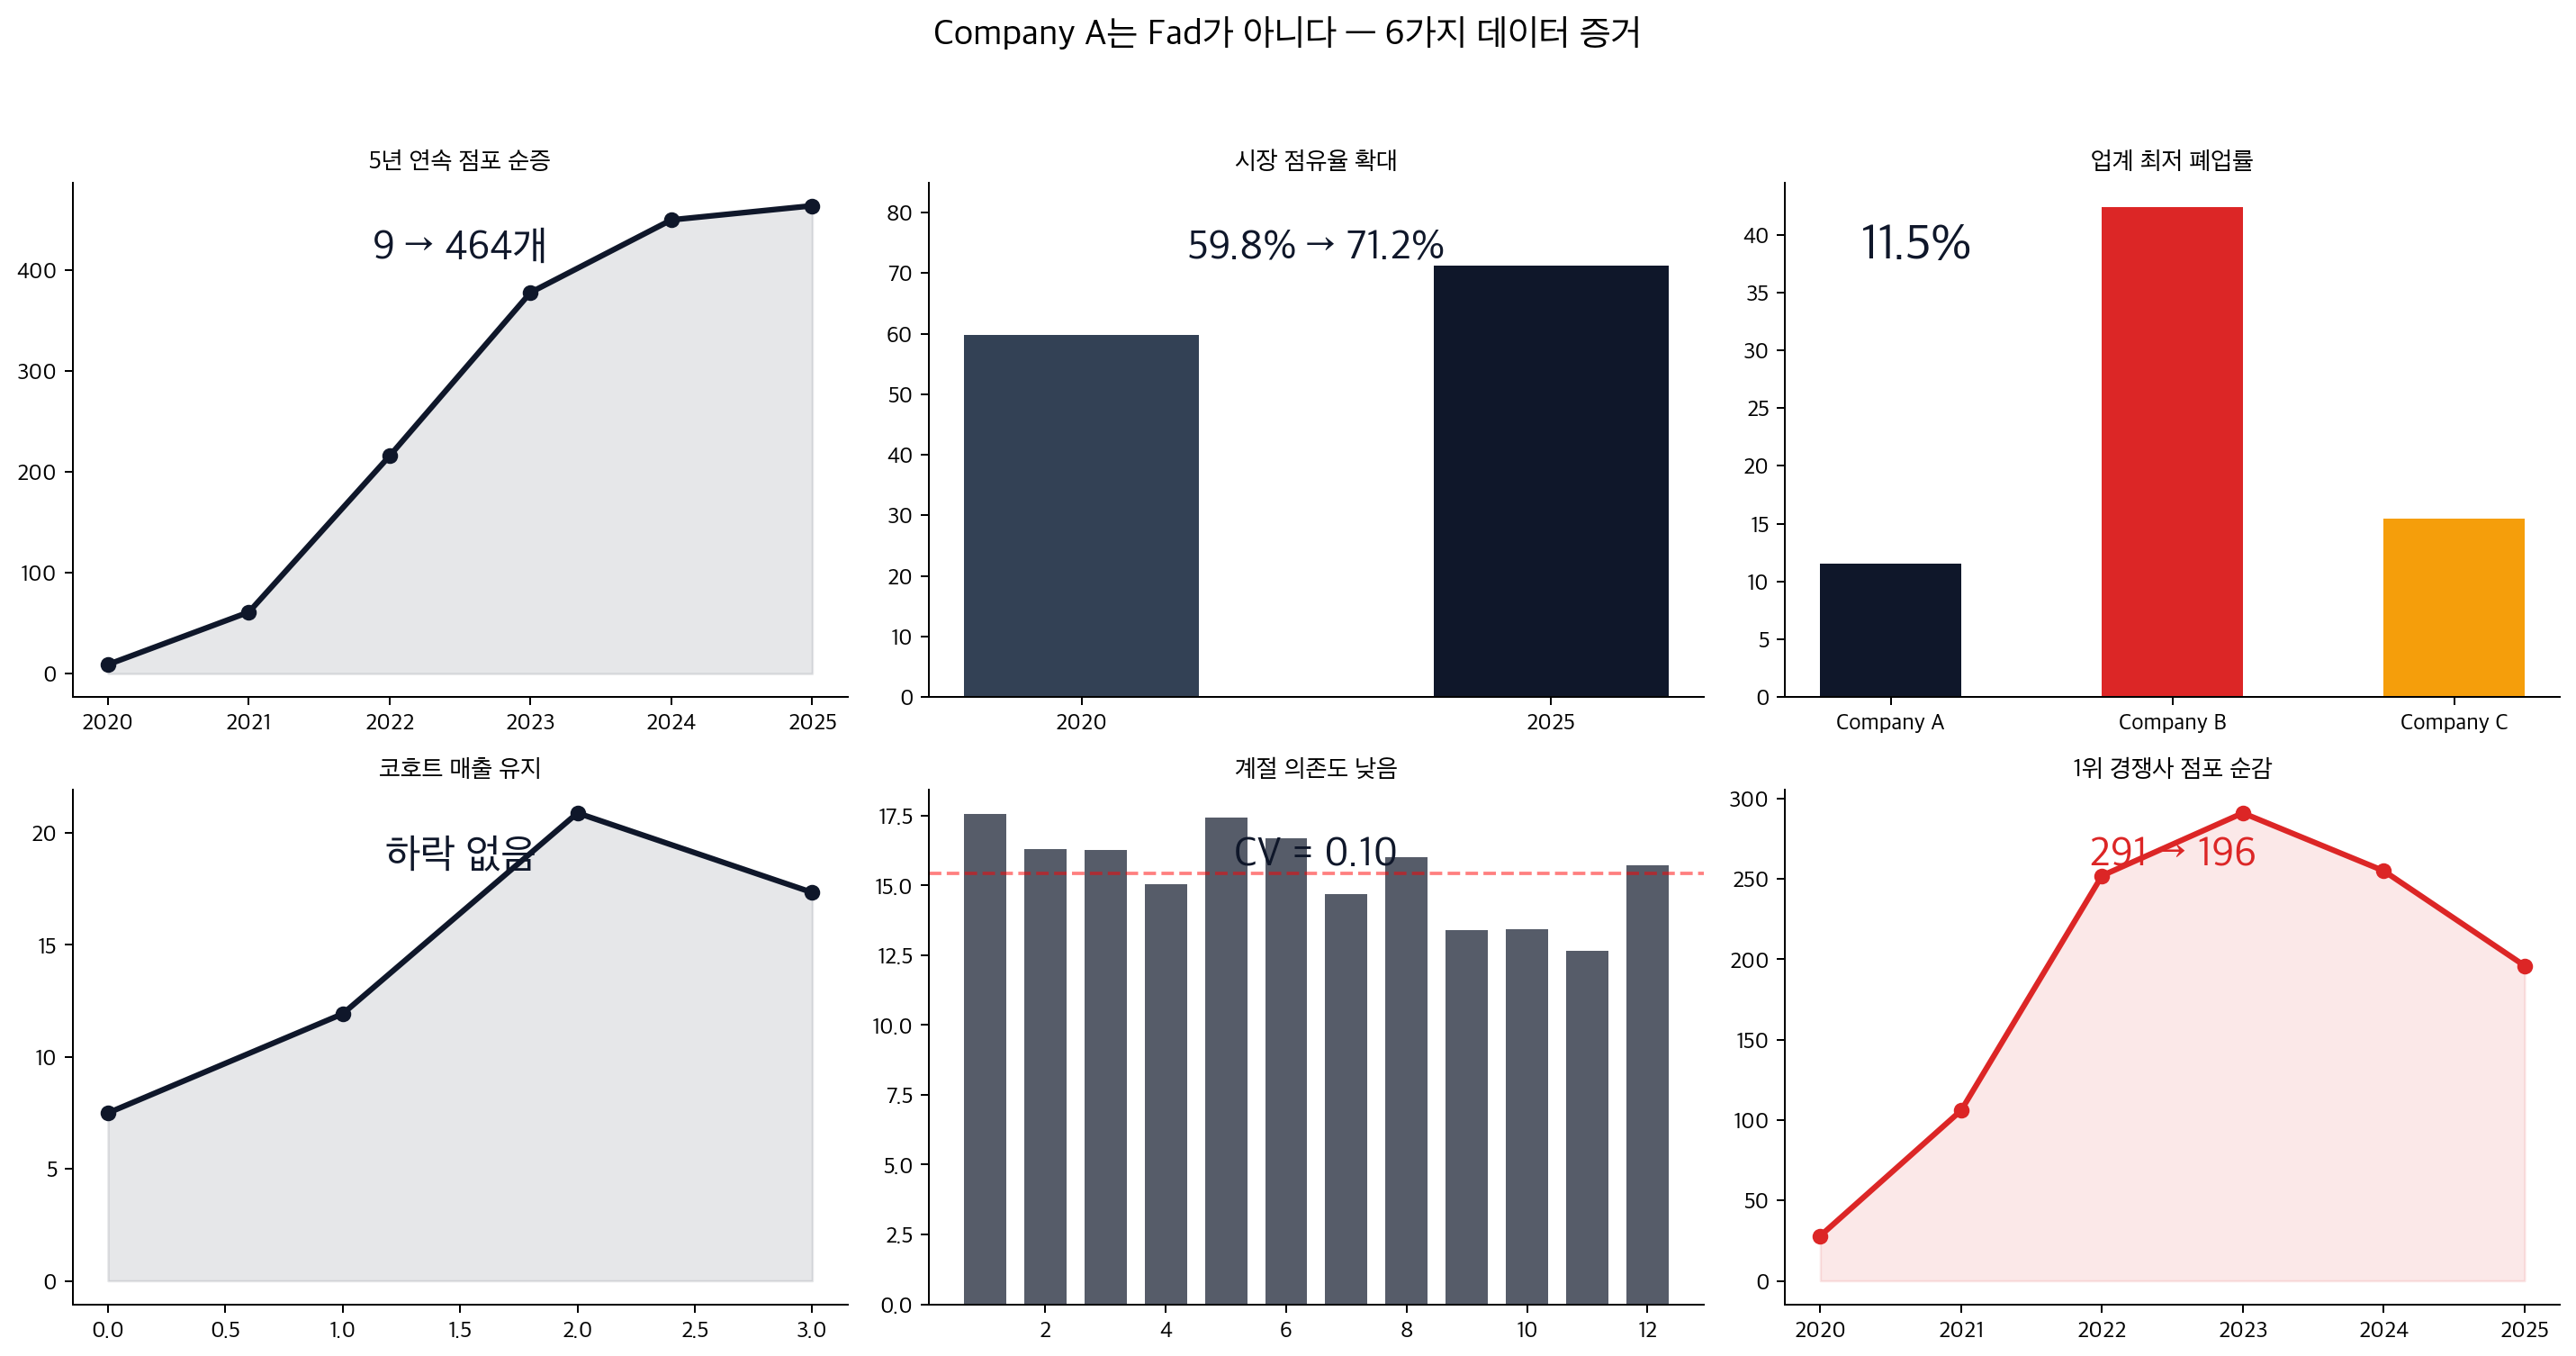
\includegraphics[width=0.95\textwidth]{B6_not_a_fad_6_evidence.png}
  \caption{셀프사진관이 일시적 유행이 아닌 6가지 증거}
\end{figure}

\vspace{0.5em}

\insightbox{순증가 매장 수, 코호트 생존율, 계절성 패턴, 시장 성숙도 지표 등 다각적 분석 결과가 모두 \textbf{구조적 성장}을 지지한다. 셀프사진관은 MZ세대의 새로운 소비 문화로 정착했다.}

\newpage

% =====================================================================
% PAGE 5: 전략적 함의
% =====================================================================
\section*{전략적 함의}

\vspace{0.5em}

본 연구 결과에서 도출된 핵심 전략적 시사점 3가지는 다음과 같다.

\vspace{1em}

\noindent
\fcolorbox{bordergray}{lightgray}{%
  \parbox{\dimexpr\textwidth-2\fboxsep-2\fboxrule}{%
    \vspace{0.8em}
    {\large\bfseries\textcolor{darkblue}{1. IP 협업은 검증된 매출 성장 전략}}\\[6pt]
    {\normalsize IP 콜라보레이션은 단기 이벤트가 아닌, 매출 증분을 실증적으로 만들어내는 핵심 성장 동력이다. MAPE 2.3\% 수준의 매출 예측 모델로 IP 협업의 ROI를 사전 추정할 수 있다.}
    \vspace{0.6em}
  }%
}

\vspace{0.8em}

\noindent
\fcolorbox{bordergray}{lightgray}{%
  \parbox{\dimexpr\textwidth-2\fboxsep-2\fboxrule}{%
    \vspace{0.8em}
    {\large\bfseries\textcolor{darkblue}{2. 경쟁사 폐업 예측으로 선제적 출점 전략 수립}}\\[6pt]
    {\normalsize AUC 0.991의 폐업 예측 모델은 경쟁사 매장의 폐업을 사전에 감지한다. 이를 통해 경쟁사 폐업 지역에 선제적으로 출점하여 시장 점유율을 확대할 수 있다.}
    \vspace{0.6em}
  }%
}

\vspace{0.8em}

\noindent
\fcolorbox{bordergray}{lightgray}{%
  \parbox{\dimexpr\textwidth-2\fboxsep-2\fboxrule}{%
    \vspace{0.8em}
    {\large\bfseries\textcolor{darkblue}{3. 시장 구조적 성장에 따른 중장기 투자 근거}}\\[6pt]
    {\normalsize 6가지 실증 증거는 셀프사진관 시장이 일시적 유행이 아님을 보여준다. 이는 중장기 투자 의사결정 및 IPO 전략 수립의 데이터 기반 근거가 된다.}
    \vspace{0.6em}
  }%
}

\vspace{2em}

\begin{figure}[H]
  \centering
  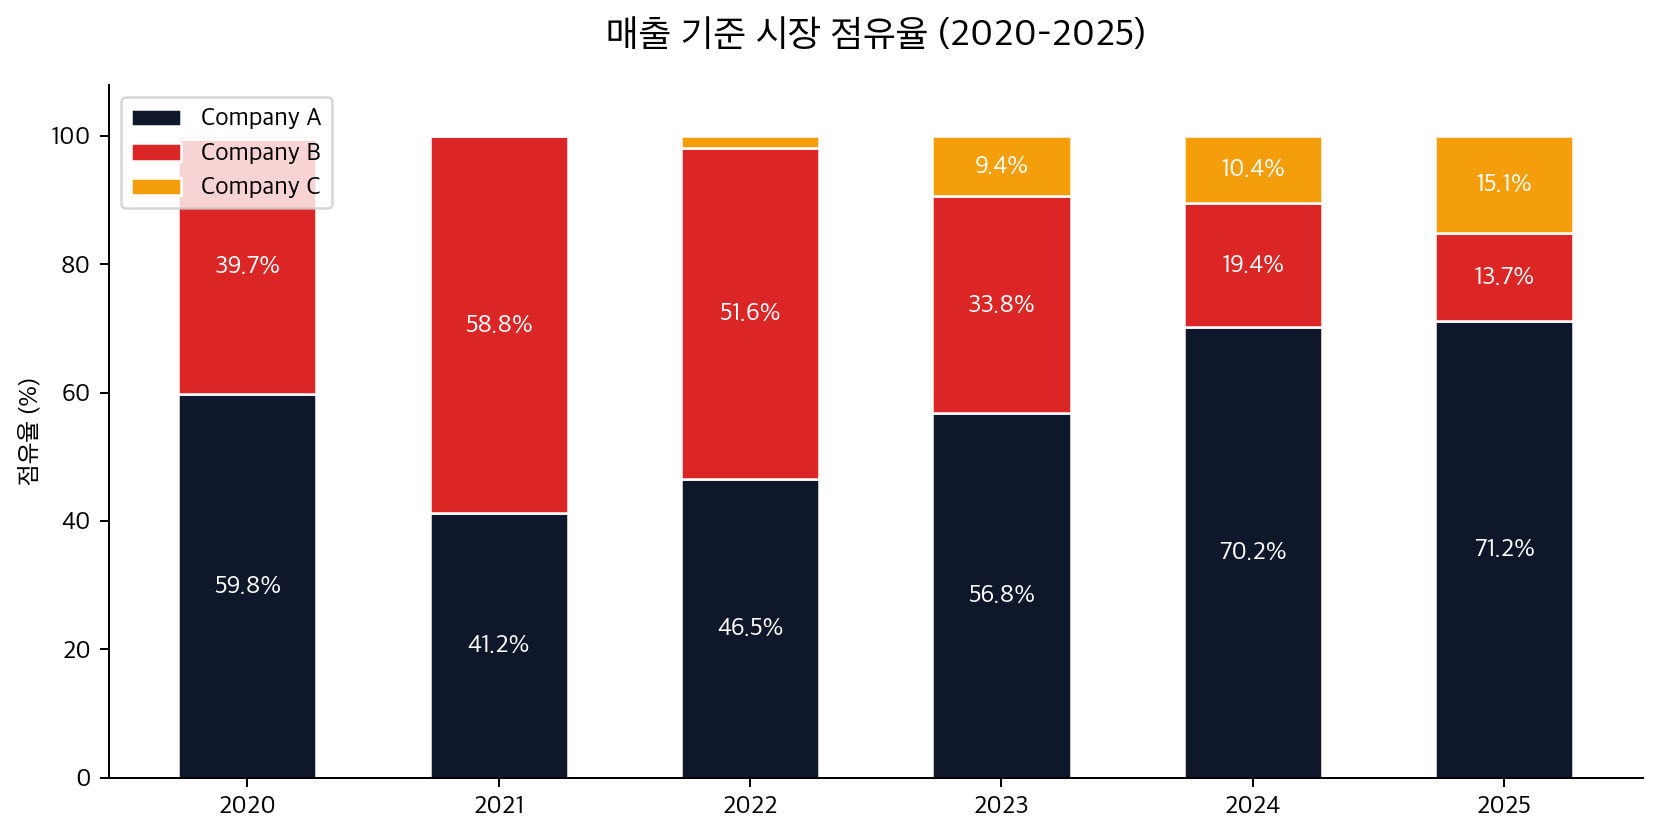
\includegraphics[width=0.85\textwidth]{A3_market_share.png}
  \caption{셀프사진관 시장 브랜드별 점유율}
\end{figure}

\newpage

% =====================================================================
% PAGE 6: 연구실 소개 + 문의
% =====================================================================
\section*{연구실 소개}

\vspace{1em}

\noindent
\fcolorbox{accent}{kpibox}{%
  \parbox{\dimexpr\textwidth-2\fboxsep-2\fboxrule}{%
    \vspace{0.8em}
    \begin{center}
    {\large\bfseries\textcolor{darkblue}{한양대학교 경영대학 임보람 교수 연구실}}\\[6pt]
    {\normalsize\textcolor{darkblue}{빅데이터 마케팅 연구그룹}}
    \end{center}
    \vspace{0.6em}
  }%
}

\vspace{1.5em}

본 연구실은 빅데이터와 머신러닝을 활용하여 기업의 마케팅 의사결정을 지원하는 실증 연구를 수행하고 있습니다. 프랜차이즈 매출 예측, 소비자 행동 분석, 시장 구조 분석 등 다양한 산업에서 데이터 기반 의사결정 모델을 개발하고 있습니다.

\vspace{1em}

\subsection*{주요 연구 분야}
\begin{itemize}[leftmargin=1.5em, itemsep=4pt]
  \item 프랜차이즈 매출 및 수요 예측
  \item 옴니채널 소비자 행동 분석
  \item 브랜드 협업(IP 콜라보레이션) 효과 측정
  \item 시장 구조 및 경쟁 분석
  \item 인구 구조 변화와 소비 트렌드 예측
\end{itemize}

\vspace{3em}

\begin{center}
\fcolorbox{darkaccent}{lightblue}{%
  \parbox{0.85\textwidth}{%
    \vspace{1em}
    \begin{center}
    {\Large\bfseries\textcolor{darkblue}{전체 보고서 및 상세 분석은}}\\[8pt]
    {\Large\bfseries\textcolor{darkblue}{연구실로 문의해주세요}}\\[12pt]
    {\normalsize\textcolor{gray}{한양대학교 경영대학 임보람 교수 연구실}}\\[4pt]
    {\normalsize\textcolor{gray}{빅데이터 마케팅 연구그룹}}
    \end{center}
    \vspace{1em}
  }%
}
\end{center}

\end{document}
